\chapter[Định luật Len-xơ về chiều dòng điện cảm ứng - Dòng điện Fu-cô]{Định luật Len-xơ về chiều dòng điện cảm ứng \\ Dòng điện Fu-cô}
\section{Lý thuyết trọng tâm}
\subsection{Định luật Len-xơ về chiều dòng điện cảm ứng }
Dòng điện cảm ứng xuất hiện trong mạch kín có chiều sao cho từ trường cảm ứng có tác dụng chống lại sự biến thiên của từ thông ban đầu qua mạch kín.

Trường hợp từ thông qua mạch biến thiên do kết quả của một chuyển động nào đó thì từ trường cảm ứng có tác dụng chống lại chuyển động nói trên. 

\subsection{Dòng điện Fu-cô (Foucault)}
\subsubsection{Định nghĩa}
Dòng điện cảm ứng được sinh ra trong khối vật dẫn khi vật dẫn chuyển động trong từ trường hay được đặt trong từ trường biến đổi theo thời gian là dòng điện Fu-cô.
\subsubsection{Tính chất của dòng điện Fu-cô}

\begin{itemize}
	\item Mọi khối kim loại chuyển động trong từ trường đều chịu tác dụng của những lực hãm điện từ. 
	\item Dòng điện Fu-cô gây ra hiệu ứng tỏa nhiệt Jun-Len-xơ: Khối kim loại chuyển động trong từ trường hoặc đặt trong từ trường biến thiên sẽ nóng lên. 
	\end{itemize}
\subsubsection{Ứng dụng của dòng điện Fu-cô}
\begin{itemize}
	\item Phanh điện từ của ô tô hạng nặng. 
	\item Lò cảm ứng để nung nóng kim loại.
	\item Dòng điện Fu-cô ứng dụng trong một số lò tôi kim loại.
\end{itemize}

Trong một số trường hợp dòng Fu-cô gây tổn hao năng lượng vô ích như làm nóng máy phát điện. Để giảm tác dụng đó của dòng điện Fu-cô, khối kim loại nguyên vẹn được thay thế bằng một khối gồm nhiều lá kim loại xếp liền nhau, cách điện với nhau. 


\section{Bài tập}
\begin{dang}{Xác định chiều dòng điện cảm ứng}
\end{dang}

\textbf{Phương pháp giải}

Áp dụng định luật Len-xơ: Dòng điện cảm ứng có chiều sao cho từ trường do nó sinh ra có tác dụng chống lại nguyên nhân sinh ra nó.

-	Nếu độ lớn từ thông \textbf{tăng}, dòng điện cảm ứng sẽ tạo ra từ trường \textbf{ngược chiều} với từ trường ban đầu.

-	Nếu độ lớn từ thông \textbf{giảm}, dòng điện cảm ứng sẽ tạo từ trường \textbf{cùng chiều} với từ trường ban đầu.

\vspace{1em}

{\viduii{2}{	
Hình vẽ nào sau đây xác định đúng chiều dòng điện cảm ứng khi cho nam châm rơi thẳng đứng xuống tâm vòng dây?
\begin{mcq}(2)
	\item 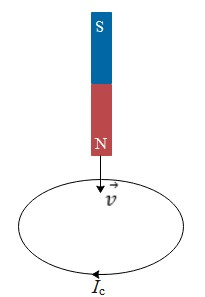
\includegraphics[scale=0.8]{../figs/VN11-PH-29-L-020-2-h65.jpg}
	\item 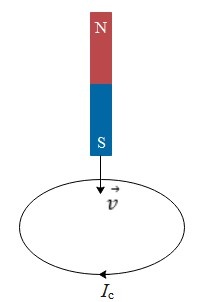
\includegraphics[scale=0.8]{../figs/VN11-PH-29-L-020-2-h68.jpg}
	\item 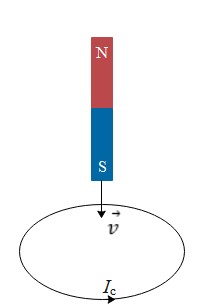
\includegraphics[scale=0.8]{../figs/VN11-PH-29-L-020-2-h67.jpg}
	\item  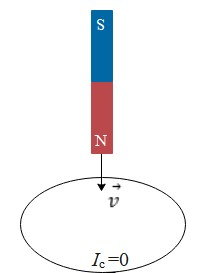
\includegraphics[scale=0.8]{../figs/VN11-PH-29-L-020-2-h66.jpg}
	
\end{mcq}}
{
\begin{center}
	\textbf{Hướng dẫn giải:}
\end{center}

Áp dụng định luật Len-xơ và quy tắc bàn tay phải.

Ở hình vẽ B nam châm đang có hướng dịch chuyển lại gần vòng dây nên từ thông nó sẽ tăng nên để chống lại sự tăng thì $\vec{B}_\text{c}$ ngược chiều $\vec{B}_\text{nam châm}$. Theo quy tắc bàn tay phải,  ta được ngón cái choãi ra chỉ chiều của $\vec{B}_\text{c}$ chiều từ cổ tay đến ngón tay chỉ chiều của $I_\text{c}$ nên nó sẽ có hướng như hình vẽ B.
	
\textbf{Đáp án: B.}}
}

{\viduii{2}
{	
Dùng định luật Len-xơ xác định chiều dòng điện cảm ứng trong khung dây dẫn khi đưa khung dây ra xa dòng điện.
\begin{center}
	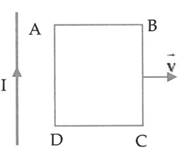
\includegraphics[scale=0.8]{../figs/VN11-PH-29-L-020-2-h69.jpg}
\end{center}}
{\begin{center}
	\textbf{Hướng dẫn giải:}
\end{center}
	\begin{center}
		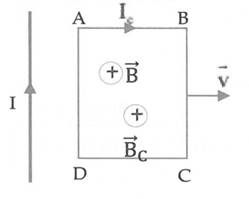
\includegraphics[scale=0.8]{../figs/VN11-PH-29-L-020-2-h70.jpg}
	\end{center}
	
Khi ta đưa khung dây ra xa dòng điện.
\begin{itemize}
	\item Cảm ứng từ $\vec{B}$ do dòng điện $I$ gây ra ở khung dây ABCD có chiều từ ngoài vào trong.
	\item Vì khung dây ra xa dòng điện $I$ nên từ thông giảm. Suy ra, từ trường cảm ứng $\vec{B}_\text{c}$ của khung dây sẽ cùng chiều với từ trường $\vec{B}$.
	\item Áp dụng quy tắc nắm bàn tay phải suy ra chiều của dòng điện cảm ứng trong khung dây ABCD có chiều từ $\text{A}\rightarrow \text{B}\rightarrow \text{C}\rightarrow \text{D}\rightarrow \text{A}$.  
\end{itemize}}
}


\begin{dang}{Dòng điện Fu-cô}
\end{dang}


{\viduii{1}{
	
	Dòng điện Fu-cô là
	\begin{mcq}
		\item dòng điện chạy trong khối vật dẫn.
		\item dòng điện cảm ứng sinh ra trong mạch kín khi từ thông qua mạch biến thiên.
		\item dòng điện cảm ứng sinh ra khi vật dẫn chuyển động trong từ trường hay được đặt trong từ trường biến đổi theo thời gian.
		\item dòng điện xuất hiện trong tấm kim loại khi nối tấm kim loại với hai cực của nguồn điện.
	\end{mcq}}
{\begin{center}
		\textbf{Hướng dẫn giải:}
\end{center}
	
	Dòng điện Fu-cô là dòng điện cảm ứng sinh ra khi vật dẫn chuyển động trong từ trường hay được đặt trong từ trường biến đổi theo thời gian.

\textbf{	Đáp án: A.}
}}

{\viduii{1}{
	
Chọn một đáp án \textbf{sai} khi nói về dòng điện Fu-cô.
\begin{mcq}
		\item Dòng điện Fu-cô gây ra hiệu ứng tỏa nhiệt.
		\item Dòng điện Fu-cô trong động cơ điện chống lại sự quay của động cơ làm giảm công suất của động cơ.
		\item Dòng điện Fu-cô trong công tơ điện có tác dụng làm cho đĩa ngừng quay nhanh khi ngắt thiết bị dùng điện.
		\item Dòng điện Fu-cô là dòng điện có hại.
	\end{mcq}}
{\begin{center}
		\textbf{Hướng dẫn giải:}
\end{center}
	
Dòng điện Fu-cô là dòng điện có hại và có lợi tùy vào các trường hợp khác nhau.
	
\textbf{	Đáp án: D.}
}}

{\viduii{1}{	
Chọn một đáp án\textbf{ sai} khi nói về dòng điện Fu-cô.
	\begin{mcq}
		\item  Hiện tượng xuất hiện dòng điện Fu-cô cô thực chất là hiện tượng cảm ứng điện từ.
		\item chiều của dòng điện Fu-cô cũng được xác định bằng định luật Jun-Lenxơ.
		\item dòng điện Fu-cô trong lõi sắt của máy biến thế là dòng điện có hại.
		\item dòng điện Fu-cô vừa có lợi và có hại.
	\end{mcq}}
{\begin{center}
		\textbf{Hướng dẫn giải:}
\end{center}
	
Chiều của dòng điện Phu cô không được xác định bằng định luật Len-xơ chứ không phải định luật Jun-Len-xơ.
	
\textbf{	Đáp án: B.}
}}




